% This section is for the experiment part of the paper, where we talk about the
% pipeline, datasets, and the models we used.

% Suggested structure:
% 1- Experiment setup/structure (pipeline)
% 2- Datasets
% 3- CC models
% 4- CLF models

\section{Experiment}

The goal of the experiment is to evaluate the effects of \gls{CC} as a pre-processing step for the cases
of simple and complex datasets and classification models. We compare it with both the base reference and a case where batch normalization is used.
Training and evaluation is done on all variations over ten trials.

For this purpose, we use two flower datasets of different complexities with 17 and 102 classes each. Our basis for comparison
are the results obtained from training and evaluating on the datasets without \gls{CC} nor batch normalization.
We then process the datasets through the different \gls{CC} methods and the batch normalization to obtain results
for the variations. For the classification of flower images, we use a fine-tuned VGG16 model and our own \gls{CNN} trained from scratch.
Figure \ref{fig:experiment_pipeline} presents an overview of the experiment.

\begin{figure}[ht]
    \centering
    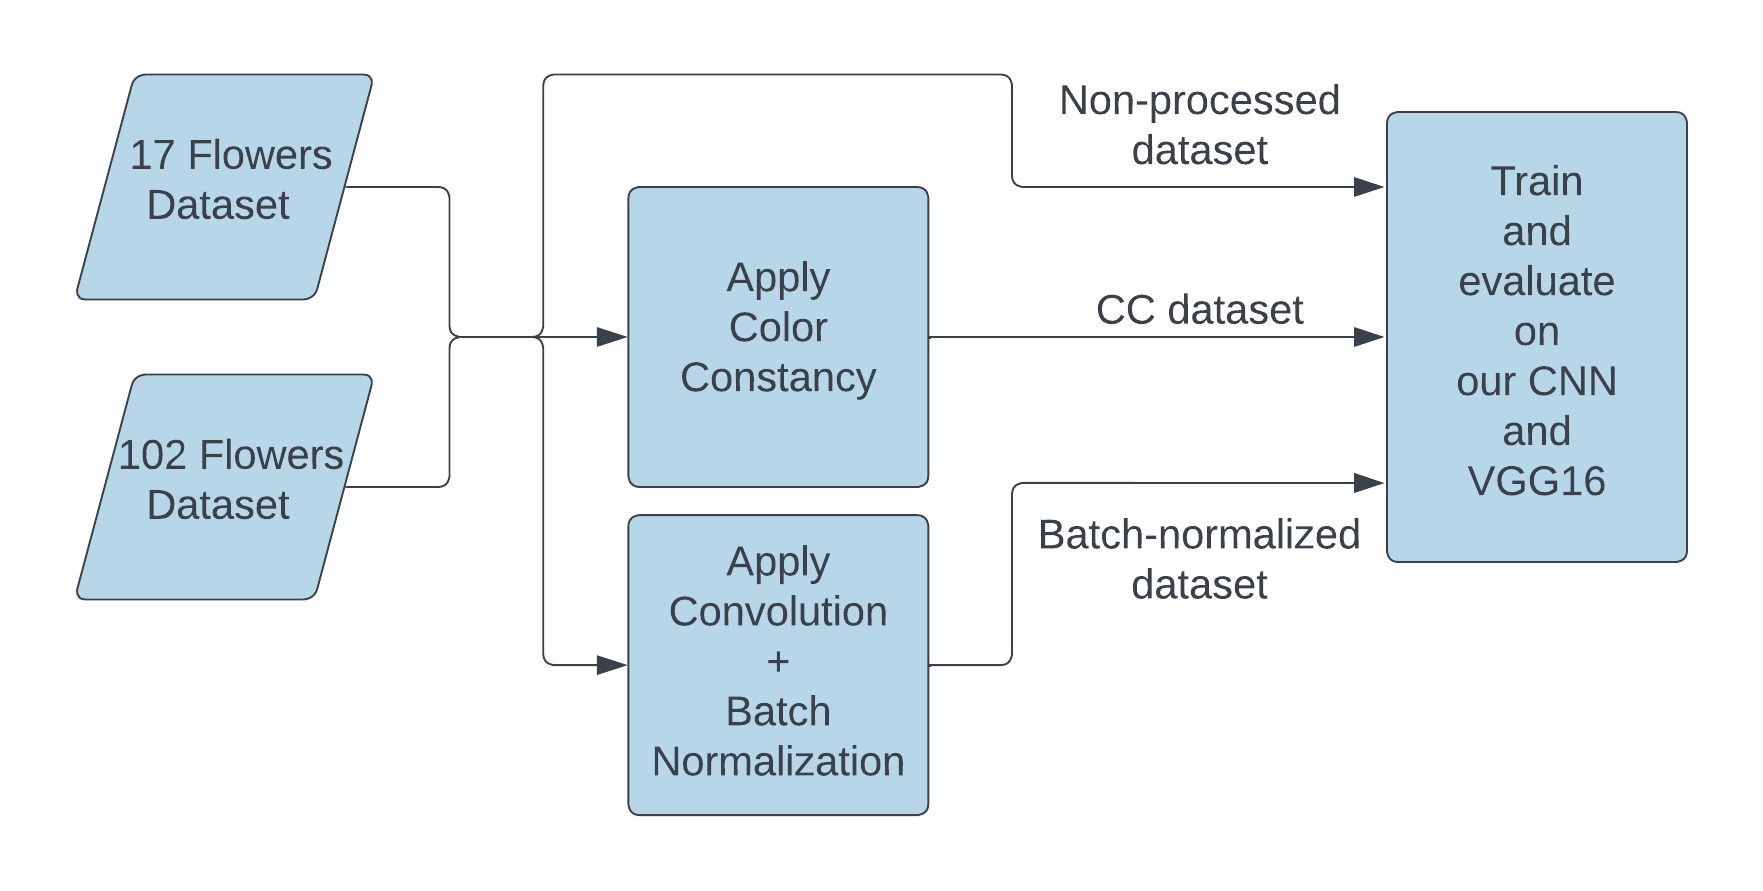
\includegraphics[width=\textwidth]{images/experiment_pipeline.png}
    \caption{Experiment overview.}
    \label{fig:experiment_pipeline}
\end{figure}

\subsection{Datasets}

We used the publicly available Oxford 17 \cite{Nilsback06} and Oxford 102 \cite{Nilsback08} flower datasets.
Oxford 17 contains 1360 images with 80 images per class, and Oxford 102 contains 8189 images with between 40 and 258 images per class.
For both datasets, we apply data augmentation by flipping the images and varying zoom, rotation, and translation.

\subsection{Color Constancy}

\begin{figure}[ht]
    \centering
    \begin{tabular}{c|cccc}
        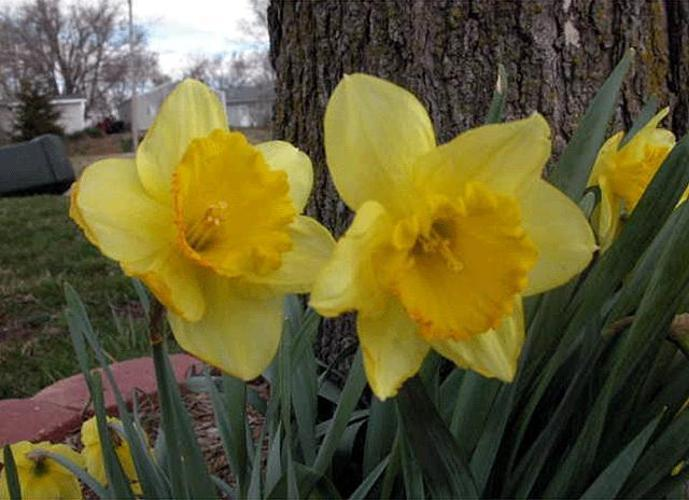
\includegraphics[width=0.165\textwidth]{cc_demo/flower001_base.png}       &
        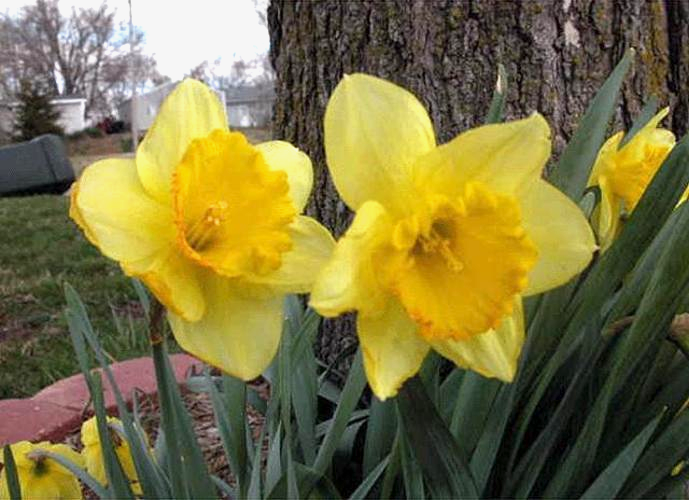
\includegraphics[width=0.165\textwidth]{cc_demo/flower001_whitePatch.png} &
        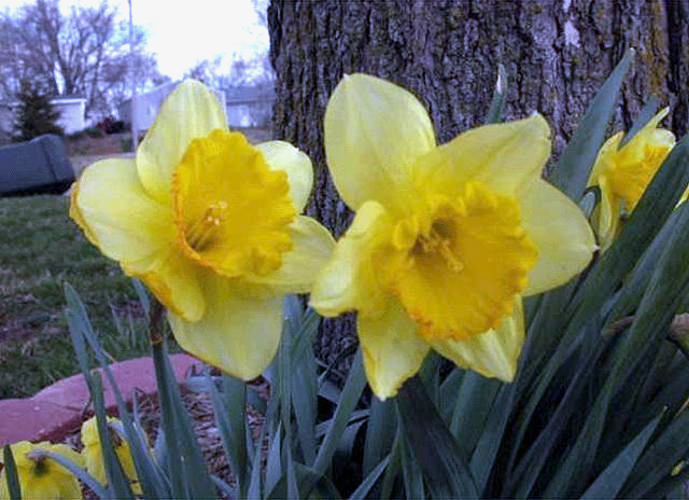
\includegraphics[width=0.165\textwidth]{cc_demo/flower001_greyWorld.png}  &
        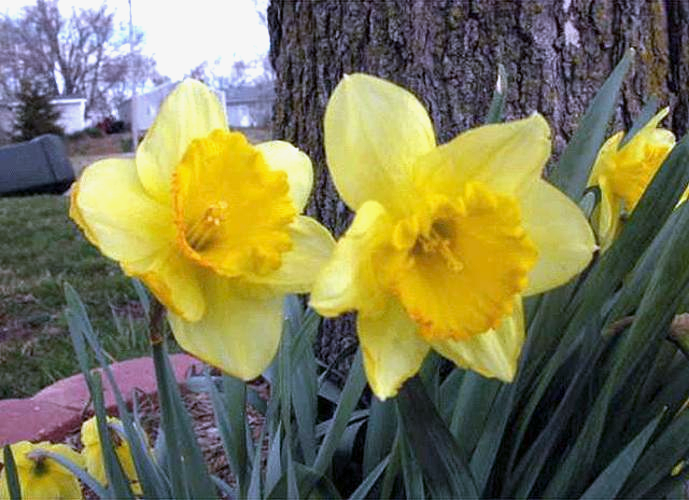
\includegraphics[width=0.165\textwidth]{cc_demo/flower001_grayEdge.png}   &
        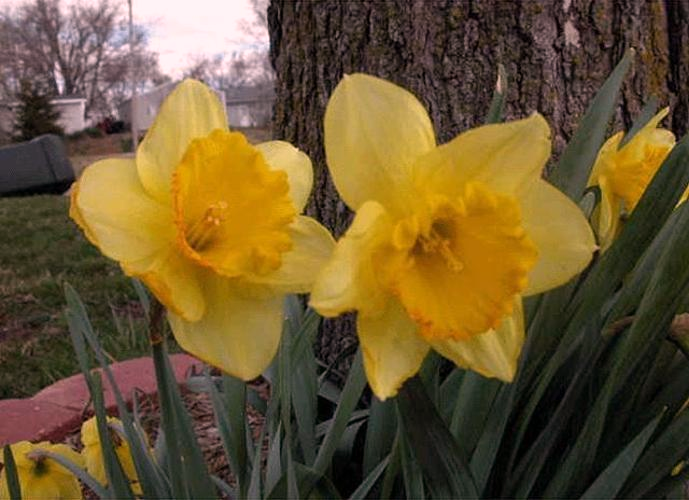
\includegraphics[width=0.165\textwidth]{cc_demo/flower001_fc4.png}                                \\
        (a)                                                                       & (b) & (c) & (d) & (e) \\
        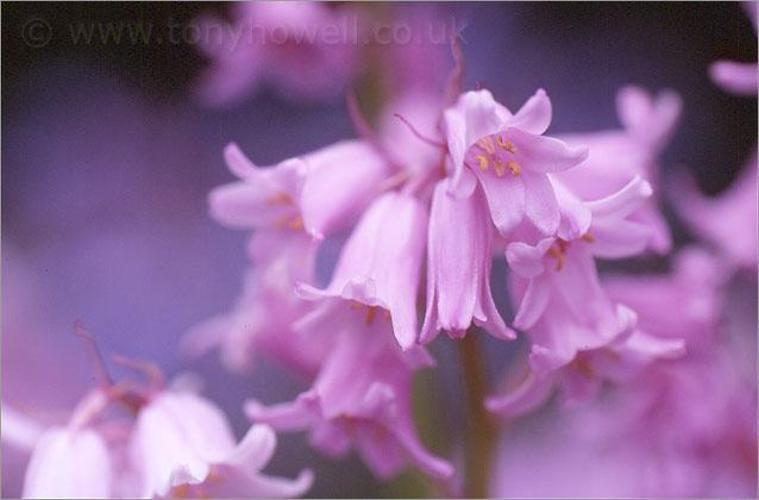
\includegraphics[width=0.165\textwidth]{cc_demo/flower268_base.png}       &
        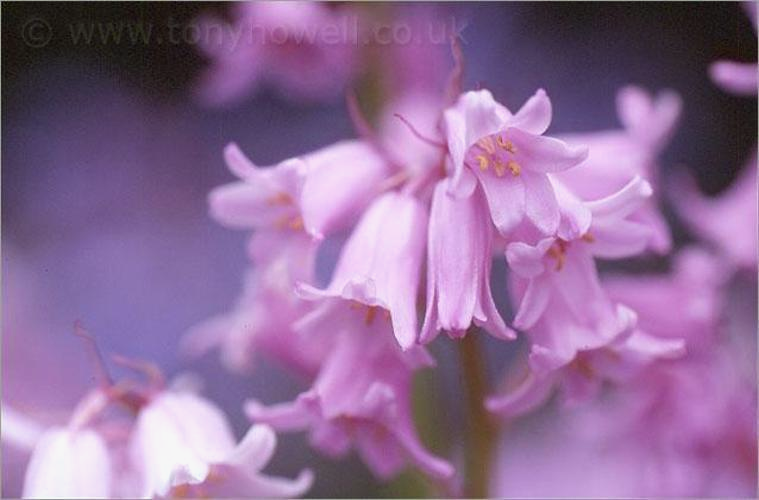
\includegraphics[width=0.165\textwidth]{cc_demo/flower268_whitePatch.png} &
        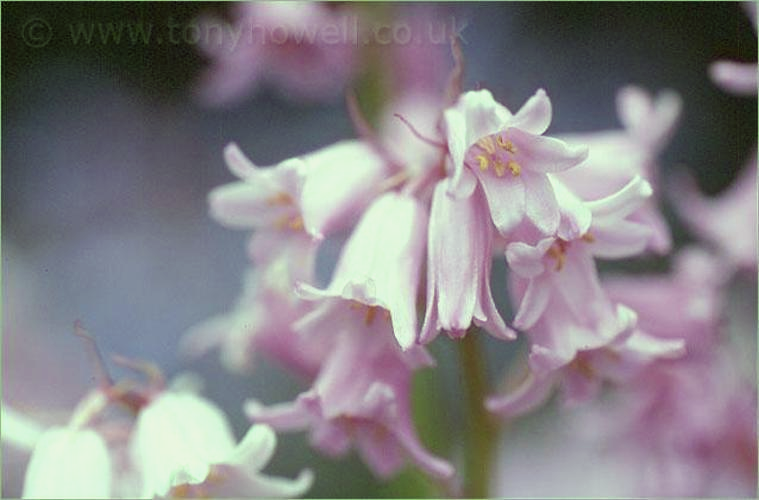
\includegraphics[width=0.165\textwidth]{cc_demo/flower268_greyWorld.png}  &
        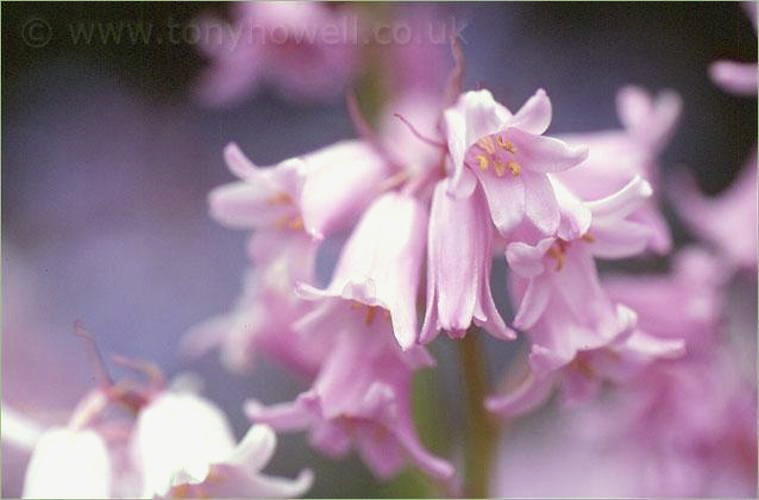
\includegraphics[width=0.165\textwidth]{cc_demo/flower268_grayEdge.png}   &
        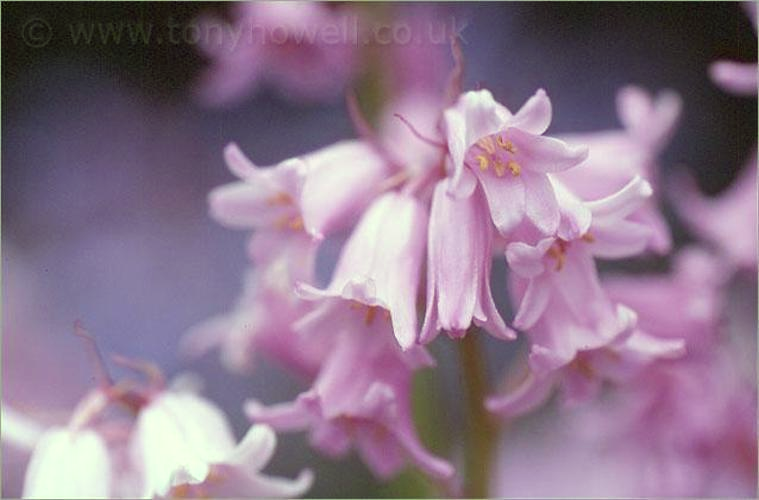
\includegraphics[width=0.165\textwidth]{cc_demo/flower268_fc4.png}                                \\
        (f)                                                                       & (g) & (h) & (i) & (j)
    \end{tabular}
    \caption{A comparison of color constancy algorithms: (a) and (f): Original image.
        (b) and (g): White Patch. (c) and (h): Grey-World.
        (d) and (i): Grey-Edge. (e) and (j): FC\textsuperscript{4}}
    \label{fig:cc_comparison}
\end{figure}

In order to have a wider spread of examined methods, we both make use of state-of-the art
learning based methods, as well as classical simpler methods
like White-Patch, Grey-World \cite{EbnerConstancy} and Grey-Edge \cite{van2005color}.
A comparison of these can be found in Figure \ref{fig:cc_comparison}.

\subsubsection{Statistical Methods}

In the grey world algorithm, the assumption is made that the average reflectance of the scene should
be a shade of grey. We can therefore infer that any deviation of the average color from this grey tone stems from
the illumination in the scene. By simply dividing this out, we receive a color-corrected image.

White-Patch is a close relative of this method, where instead we assume that the brightest spot in the image (for each channel)
is representative of the overall light color.

In the grey-edge hypothesis we instead assume that the average image gradient can be used as an indication of the light color.

All of these algorithms were reimplemented by us. Notably, based on the recommendation made by Ebner \cite{EbnerConstancy},
after color adjustment we rescale all results such that the top 5\% of values (across all channels) will be clipped to
the maximum intensity of 1.

\subsubsection{Learning Based Model}

We use the FC\textsuperscript{4} model\cite{hu2017fc} as our representative for the deep learning based models. This is a considerably more complicated approach
than the statistical methods listed above, as it makes use of deep convolutional networks.

We chose FC\textsuperscript{4}, as it can provide us with high quality outputs, while still being reasonably simple to use within our framework. While newer
models might perform slightly better when evaluated purely on their results, we judged that FC\textsuperscript{4} should already provide a sufficiently large\
delta to the statistical methods to give an indication of whether this approach is worth pursuing.

\subsection{Classification models}

In this study, two distinct classification models were employed: a pre-trained VGG16 and our own \gls{CNN} trained from scratch.
To ensure a standardized approach for fair comparison and evaluation, certain key methodologies were incorporated.
Specifically, we applied consistent RMSProp optimizer and Sparse Cross Entropy loss function across both models.
Given that we have 17 and 102 flower categories, this loss function is suitable for our multi-class classification problem. Moreover, to explore different optimization paths, we set the learning rate
for our custome model as 1e-3 and 1e-4 for the Pre-trained VGG16 model.

\subsubsection{VGG16}
The VGG16 model \cite{SimonyanVGG} well-known for its simplicity and effectiveness in image classification tasks \cite{SimonyanVGG} is used as a feature extractor in our study. Pre-trained on the ImageNet dataset, it effectively captures high-level features.
By utilizing transfer learning, we take advantage of the pre-trained weights of the VGG16 model that were trained on the large-scale ImageNet dataset.

The last four layers are fine-tuned for our flower classification, while the first layers remain frozen to preserve latent features. The final layer is replaced with a new fully connected layer of 17 or 102 neurons (depending on which dataset is being used) and SoftMax activation function.
And a flatten layer that converts the output into a one-dimensional feature vector, followed by a dense layer of 1024 neurons and a dropout layer to prevent overfitting \cite{kaggle_flower_cnn}.

\subsubsection{Our CNN}

The implemented \gls{CNN} consists of pairs of convolutions and max pooling, followed by a flatten, ReLU activation, dropout, and a fully-connected dense layer for classification.
The \gls{CC} layer is included before the first convolution, and the batch normalization layer is in-between the first convolution (input layer) and it's ReLU activation.
It is a simple network designed to score well on the Oxford 17 dataset (approximatelly $80\%$ test accuracy). Figure \ref{fig:our_cnn} shows the implemented architecture with the batch normalization layer.


\begin{figure}[ht]
    \centering
    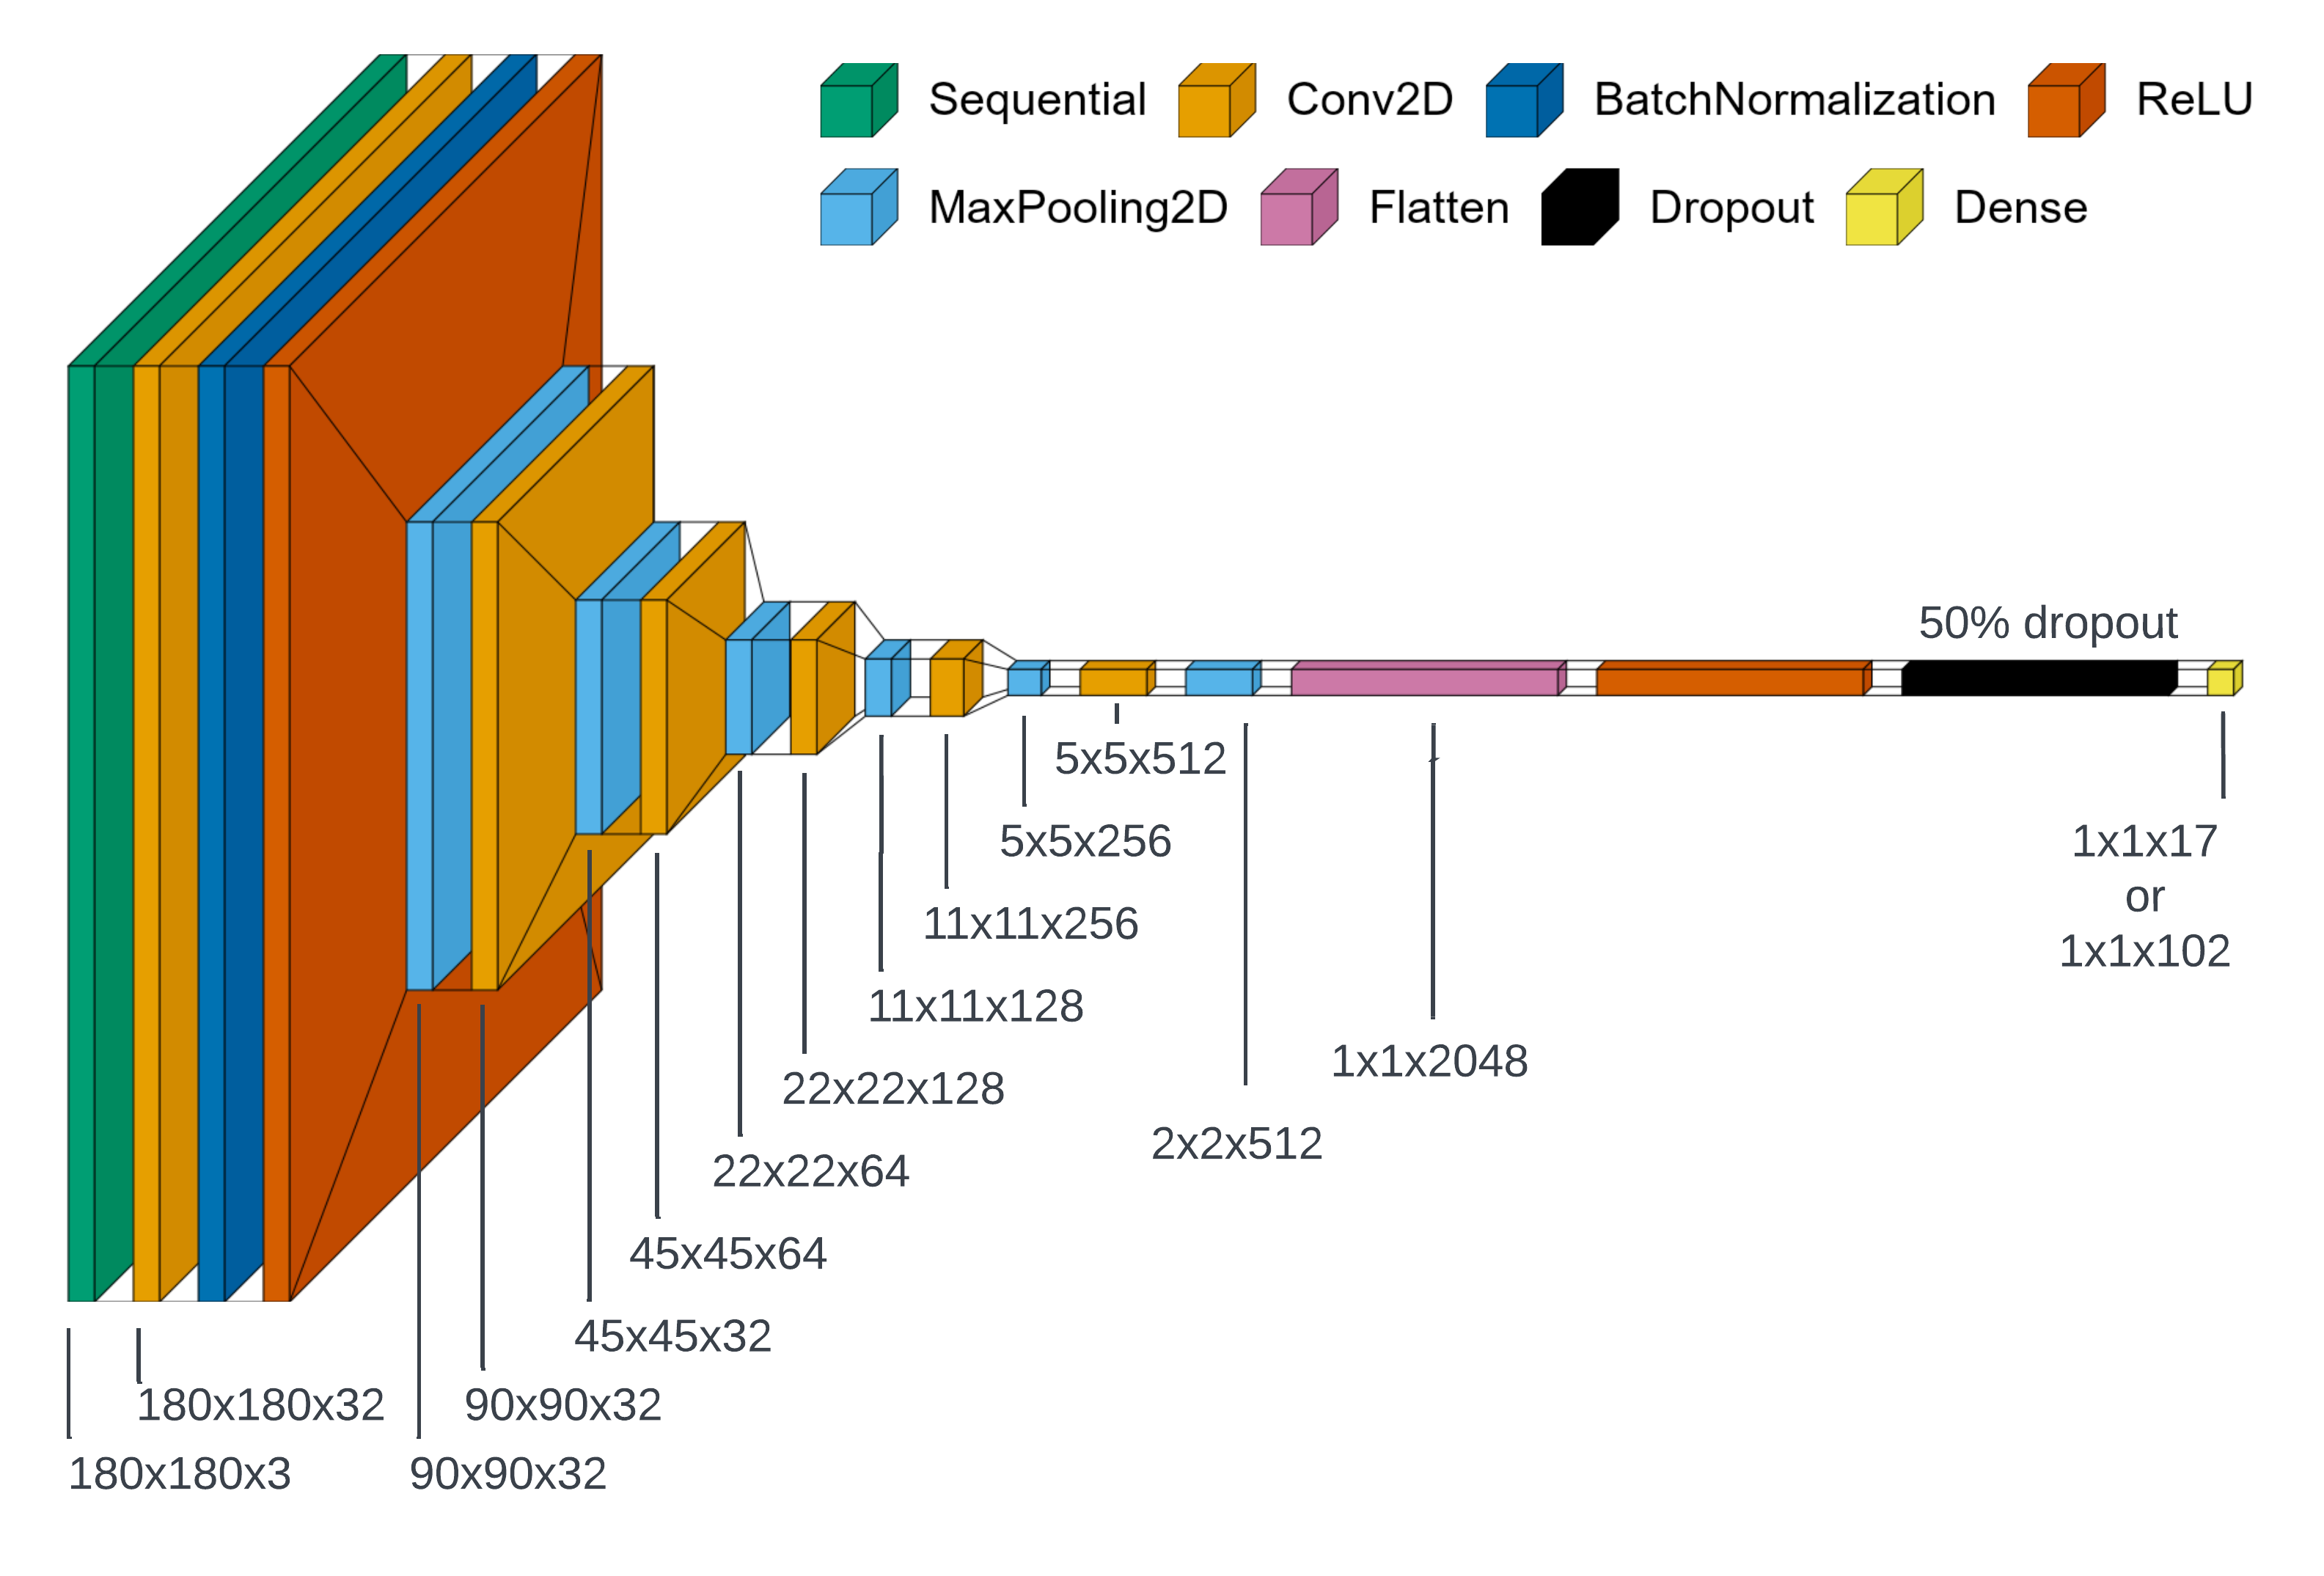
\includegraphics[width=\textwidth]{images/ours_architecture.png}
    \caption{Architecture of our CNN.}
    \label{fig:our_cnn}
\end{figure}